% Created by tikzDevice version 0.12.4 on 2023-11-07 16:58:59
% !TEX encoding = UTF-8 Unicode
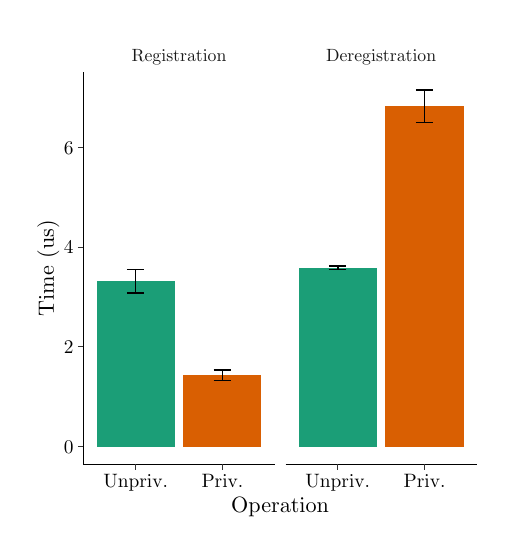
\begin{tikzpicture}[x=1pt,y=1pt]
\definecolor{fillColor}{RGB}{255,255,255}
\path[use as bounding box,fill=fillColor,fill opacity=0.00] (0,0) rectangle (166.22,180.67);
\begin{scope}
\path[clip] (  0.00,  0.00) rectangle (166.22,180.67);
\definecolor{drawColor}{RGB}{255,255,255}
\definecolor{fillColor}{RGB}{255,255,255}

\path[draw=drawColor,line width= 0.4pt,line join=round,line cap=round,fill=fillColor] (  0.00,  0.00) rectangle (166.22,180.68);
\end{scope}
\begin{scope}
\path[clip] ( 20.16, 22.85) rectangle ( 89.19,164.62);
\definecolor{fillColor}{RGB}{255,255,255}

\path[fill=fillColor] ( 20.16, 22.85) rectangle ( 89.19,164.62);
\definecolor{fillColor}{RGB}{217,95,2}

\path[fill=fillColor] ( 56.25, 29.29) rectangle ( 84.49, 55.10);
\definecolor{fillColor}{RGB}{27,158,119}

\path[fill=fillColor] ( 24.87, 29.29) rectangle ( 53.11, 89.00);
\definecolor{drawColor}{RGB}{0,0,0}

\path[draw=drawColor,line width= 0.6pt,line join=round] ( 67.23, 57.08) --
	( 73.50, 57.08);

\path[draw=drawColor,line width= 0.6pt,line join=round] ( 70.37, 57.08) --
	( 70.37, 53.13);

\path[draw=drawColor,line width= 0.6pt,line join=round] ( 67.23, 53.13) --
	( 73.50, 53.13);

\path[draw=drawColor,line width= 0.6pt,line join=round] ( 35.85, 93.30) --
	( 42.13, 93.30);

\path[draw=drawColor,line width= 0.6pt,line join=round] ( 38.99, 93.30) --
	( 38.99, 84.70);

\path[draw=drawColor,line width= 0.6pt,line join=round] ( 35.85, 84.70) --
	( 42.13, 84.70);
\end{scope}
\begin{scope}
\path[clip] ( 93.19, 22.85) rectangle (162.22,164.62);
\definecolor{fillColor}{RGB}{255,255,255}

\path[fill=fillColor] ( 93.19, 22.85) rectangle (162.22,164.62);
\definecolor{fillColor}{RGB}{27,158,119}

\path[fill=fillColor] ( 97.90, 29.29) rectangle (126.14, 93.85);
\definecolor{fillColor}{RGB}{217,95,2}

\path[fill=fillColor] (129.28, 29.29) rectangle (157.51,152.28);
\definecolor{drawColor}{RGB}{0,0,0}

\path[draw=drawColor,line width= 0.6pt,line join=round] (108.88, 94.45) --
	(115.16, 94.45);

\path[draw=drawColor,line width= 0.6pt,line join=round] (112.02, 94.45) --
	(112.02, 93.25);

\path[draw=drawColor,line width= 0.6pt,line join=round] (108.88, 93.25) --
	(115.16, 93.25);

\path[draw=drawColor,line width= 0.6pt,line join=round] (140.26,158.18) --
	(146.53,158.18);

\path[draw=drawColor,line width= 0.6pt,line join=round] (143.40,158.18) --
	(143.40,146.39);

\path[draw=drawColor,line width= 0.6pt,line join=round] (140.26,146.39) --
	(146.53,146.39);
\end{scope}
\begin{scope}
\path[clip] ( 20.16,164.62) rectangle ( 89.19,176.68);
\definecolor{drawColor}{gray}{0.10}

\node[text=drawColor,anchor=base,inner sep=0pt, outer sep=0pt, scale=  0.64] at ( 54.68,168.45) {Registration};
\end{scope}
\begin{scope}
\path[clip] ( 93.19,164.62) rectangle (162.22,176.68);
\definecolor{drawColor}{gray}{0.10}

\node[text=drawColor,anchor=base,inner sep=0pt, outer sep=0pt, scale=  0.64] at (127.71,168.45) {Deregistration};
\end{scope}
\begin{scope}
\path[clip] (  0.00,  0.00) rectangle (166.22,180.67);
\definecolor{drawColor}{RGB}{0,0,0}

\path[draw=drawColor,line width= 0.6pt,line join=round] ( 20.16, 22.85) --
	( 89.19, 22.85);
\end{scope}
\begin{scope}
\path[clip] (  0.00,  0.00) rectangle (166.22,180.67);
\definecolor{drawColor}{gray}{0.20}

\path[draw=drawColor,line width= 0.4pt,line join=round] ( 38.99, 20.85) --
	( 38.99, 22.85);

\path[draw=drawColor,line width= 0.4pt,line join=round] ( 70.37, 20.85) --
	( 70.37, 22.85);
\end{scope}
\begin{scope}
\path[clip] (  0.00,  0.00) rectangle (166.22,180.67);
\definecolor{drawColor}{RGB}{0,0,0}

\node[text=drawColor,anchor=base,inner sep=0pt, outer sep=0pt, scale=  0.70] at ( 38.99, 14.43) {Unpriv.};

\node[text=drawColor,anchor=base,inner sep=0pt, outer sep=0pt, scale=  0.70] at ( 70.37, 14.43) {Priv.};
\end{scope}
\begin{scope}
\path[clip] (  0.00,  0.00) rectangle (166.22,180.67);
\definecolor{drawColor}{RGB}{0,0,0}

\path[draw=drawColor,line width= 0.6pt,line join=round] ( 93.19, 22.85) --
	(162.22, 22.85);
\end{scope}
\begin{scope}
\path[clip] (  0.00,  0.00) rectangle (166.22,180.67);
\definecolor{drawColor}{gray}{0.20}

\path[draw=drawColor,line width= 0.4pt,line join=round] (112.02, 20.85) --
	(112.02, 22.85);

\path[draw=drawColor,line width= 0.4pt,line join=round] (143.40, 20.85) --
	(143.40, 22.85);
\end{scope}
\begin{scope}
\path[clip] (  0.00,  0.00) rectangle (166.22,180.67);
\definecolor{drawColor}{RGB}{0,0,0}

\node[text=drawColor,anchor=base,inner sep=0pt, outer sep=0pt, scale=  0.70] at (112.02, 14.43) {Unpriv.};

\node[text=drawColor,anchor=base,inner sep=0pt, outer sep=0pt, scale=  0.70] at (143.40, 14.43) {Priv.};
\end{scope}
\begin{scope}
\path[clip] (  0.00,  0.00) rectangle (166.22,180.67);
\definecolor{drawColor}{RGB}{0,0,0}

\path[draw=drawColor,line width= 0.6pt,line join=round] ( 20.16, 22.85) --
	( 20.16,164.62);
\end{scope}
\begin{scope}
\path[clip] (  0.00,  0.00) rectangle (166.22,180.67);
\definecolor{drawColor}{RGB}{0,0,0}

\node[text=drawColor,anchor=base east,inner sep=0pt, outer sep=0pt, scale=  0.70] at ( 16.56, 26.88) {0};

\node[text=drawColor,anchor=base east,inner sep=0pt, outer sep=0pt, scale=  0.70] at ( 16.56, 62.91) {2};

\node[text=drawColor,anchor=base east,inner sep=0pt, outer sep=0pt, scale=  0.70] at ( 16.56, 98.93) {4};

\node[text=drawColor,anchor=base east,inner sep=0pt, outer sep=0pt, scale=  0.70] at ( 16.56,134.96) {6};
\end{scope}
\begin{scope}
\path[clip] (  0.00,  0.00) rectangle (166.22,180.67);
\definecolor{drawColor}{gray}{0.20}

\path[draw=drawColor,line width= 0.4pt,line join=round] ( 18.16, 29.29) --
	( 20.16, 29.29);

\path[draw=drawColor,line width= 0.4pt,line join=round] ( 18.16, 65.32) --
	( 20.16, 65.32);

\path[draw=drawColor,line width= 0.4pt,line join=round] ( 18.16,101.34) --
	( 20.16,101.34);

\path[draw=drawColor,line width= 0.4pt,line join=round] ( 18.16,137.37) --
	( 20.16,137.37);
\end{scope}
\begin{scope}
\path[clip] (  0.00,  0.00) rectangle (166.22,180.67);
\definecolor{drawColor}{RGB}{0,0,0}

\node[text=drawColor,anchor=base,inner sep=0pt, outer sep=0pt, scale=  0.80] at ( 91.19,  5.56) {Operation};
\end{scope}
\begin{scope}
\path[clip] (  0.00,  0.00) rectangle (166.22,180.67);
\definecolor{drawColor}{RGB}{0,0,0}

\node[text=drawColor,rotate= 90.00,anchor=base,inner sep=0pt, outer sep=0pt, scale=  0.80] at (  9.51, 93.73) {Time (us)};
\end{scope}
\end{tikzpicture}
